% uw-wkrpt-se.tex - An example work report that uses uw-wkrpt.cls
% Copyright (C) 2002,2003  Simon Law
% 
% This program is free software; you can redistribute it and/or modify
% it under the terms of the GNU General Public License as published by
% the Free Software Foundation; either version 2 of the License, or
% (at your option) any later version.
% 
% This program is distributed in the hope that it will be useful,
% but WITHOUT ANY WARRANTY; without even the implied warranty of
% MERCHANTABILITY or FITNESS FOR A PARTICULAR PURPOSE.  See the
% GNU General Public License for more details.
% 
% You should have received a copy of the GNU General Public License
% along with this program; if not, write to the Free Software
% Foundation, Inc., 59 Temple Place, Suite 330, Boston, MA  02111-1307  USA
%
%%%%%%%%%%%%%%%%%%%%%%%%%%%%%%%%%%%%%%%%%%%%%%%%%%%%%%%%%%%%%%%%%%%%%
%
% We begin by calling the workreport class which includes all the
% definitions for the macros we will use.
\documentclass[se,blockletter]{uw-wkrpt}

% LaTeX preamble: load some packages to add functionality
\usepackage{graphicx} % Include graphic importing

\usepackage[T1]{fontenc} % Better fonts
\usepackage{ae,aecompl}

\usepackage{indentfirst} % Indent first paragraph of each section

% Use biblatex for references
\usepackage[style=ieee,sorting=none,dateabbrev=false]{biblatex}
\addbibresource{uw-wkrpt-bib.bib} % Specify the bibliography file

% This needs to be the last package loaded
\usepackage[pdftex]{hyperref} % Generate PDF links and bookmarks.
\hypersetup{
  bookmarks=true,
  bookmarksnumbered=true
}

% Now we will begin writing the document.
\begin{document}

%%%%%%%%%%%%%%%%%%%%%%%%%%%%%%%%%%%%%%%%%%%%%%%%%%%%%%%%%%%%%%%%%%%%%
%% IMPORTANT INFORMATION
%%%%%%%%%%%%%%%%%%%%%%%%%%%%%%%%%%%%%%%%%%%%%%%%%%%%%%%%%%%%%%%%%%%%%

%% First we, should create a title page.  This is done below:
% Fill in the title of your report.
\title{Application of Machine Learning Models as a Solution to Hyperbola Identification in Ground Penetrating Radar Data}

% Fill in your name.
\author{Xiang Yi (Irene) Chen}

% Fill in your student ID number.
\uwid{20707344}

% Fill in your home address.
\address{277 Lester Street \\*
         Waterloo, ON\ \ N2L 3W6}

% Fill in your employer's name.
\employer{Sensors \& Software Inc.}

% Fill in your employer's city and province.
\employeraddress{Mississauga, ON}

% Fill in your school's name.
\school{University of Waterloo}

% Fill in your faculty name.
\faculty{Software Engineering}

% Fill in your student user ID
\userid{xy29chen}

% Fill in your e-mail address.
\email{irene.chen@edu.uwaterloo.ca}

% Fill in your term.
\term{1B}

% Fill in your program.
\program{Software Engineering}

% Fill in the department chair's name.
\chair{Dr.\ D.\ Rayside}

% Fill in the department chair's mailing address.
\chairaddress{Software Engineering\\*
              University of Waterloo\\*
	      	 Waterloo, ON\ \ N2L 3G1}

% If you are writing an "SE-confidential" report, uncomment the next line.
%\confidential{SE-confidential}

% If you want to specify the date, fill it in here.  If you comment out
% this line, today's date will be substituted.
\date{August 17, 2018}

% Now, we ask LaTeX to generate the title.
\maketitle


\newcommand{\thecompany}{Sensors \& Software Inc.}

%%%%%%%%%%%%%%%%%%%%%%%%%%%%%%%%%%%%%%%%%%%%%%%%%%%%%%%%%%%%%%%%%%%%%
%% FRONT MATTER
%%%%%%%%%%%%%%%%%%%%%%%%%%%%%%%%%%%%%%%%%%%%%%%%%%%%%%%%%%%%%%%%%%%%%
%% \frontmatter will make the \section commands ignore their numbering,
%% it will also use roman page numbers.
\frontmatter

% After this, we must create a letter of submission.
\begin{letter}

The following work term report, entitled ``\thetitle'', has been prepared for \theemployer{} as my first work term report for my \theterm{} term. The objective of this work term report is to explore the feasibility of different machine learning models to the problem of hyperbola recognition and classification, in ground penetrating radar data. 

\theemployer{} is a major provider in ground penetrating radars, both software and hardware.

I would like to thank my supervisor, Adam Fazzari for providing support and guidance along the way, as well as my co-workers for furthering my understanding of ground penetrating radars, from usage to data interpretation. Finally I would like to thank \theemployer{} for providing for the data set and other resources needed to retrain the models. 

% Note that I do not need to type out the boilerplate confirmation,
% nor do I need to write a signature block.  This is generated for me.
% We are now finished with the letter.
\end{letter}

% We continue with required sections, such as the Executive Summary.
\section{Executive Summary}
The following report investigates the suitability of a small sample of pre-trained machine learning models, in response to the challenge of identifying hyperbolas in ground penetrating radar (GPR). The problem stems from the fact that hyperbola artefacts in GPR data are highly contextual, and present themselves in many different forms. As such, streamlining the interpretation process with software aids for GPR users proves itself to be a challenge, due to this visual variety in the data.

However, the identification of hyperbola may be solved with the use of machine learning training. Hence, the Inception V3 model, as well as MobileNet V2 model, and VGG 19 model will be compared to determine their suitability given restrictions to this identification problem, and ultimately proven by a proof-of-concept application to hyperbola identification.

\subsection{Disclaimer}
The pre-trained models and their retraining modules are publicly available on GitHub. They've been applied with proprietary GPR data provided by \thecompany{}  

% Next, we need to make a Table of Contents, List of Figures and 
% List of Tables.  You will most likely need to run LaTeX twice to
% get these correct.  The first pass for LaTeX to figure out the
% labels, and the second pass to put in the right references.
\tableofcontents
\listoffigures
\listoftables

%%%%%%%%%%%%%%%%%%%%%%%%%%%%%%%%%%%%%%%%%%%%%%%%%%%%%%%%%%%%%%%%%%%%%
%% REPORT BODY
%%%%%%%%%%%%%%%%%%%%%%%%%%%%%%%%%%%%%%%%%%%%%%%%%%%%%%%%%%%%%%%%%%%%%
%% \main will make the \section commands numbered again,
%% it will also use arabic page numbers.
\mainmatter

% You must have an Introduction
\section{Introduction}\label{sec:intro}
Ground Penetrating Radar (GPR) solutions serve a wide range of uses, from underground utility locating, to pavement or ice thickness mapping, to forensics as well as archaeology. However, because of this varied usage---combined with pre-processing and post-processing---GPR data presents itself in many various ways. Hence, interpretation of GPR data is one of the most error-prone aspects of using GPR solutions.

\subsection{Problem Statement}
One of the biggest challenges of GPR data interpretation is to avoid false positives, such as extreme ringing caused by metal, 
as well as interference caused by rebounding air waves off the data collection site.

\thecompany{}'s software is able to apply velocity fitting and other transformations to GPR data to improve and simplify data interpretation, such as identifying false-positive air waves in GPR data through a calculation of its velocity. However, the first and most limiting step to this process is to allow the software to locate hyperbola---evidence of a disturbance in the soil caused by an object. 

\subsection{Proposal of Solution}
Since machine learning has been making advances in the field of computer vision, it seems to be a fit tool to solve this bottleneck in this interpretation process.

Machine learning, in the broadest of terms, is a subset of computer science which allows programs to improve and "learn" without explicitly being told what exactly to do---the construction of algorithms to make predictions based on recognition of patterns on a data set and to make changes to itself so that its future performance is improved. 

Specifically, object detection and localization problems generally involve training feature extraction: associating certain characteristics of the image with different weights of importance based on their reoccurrence. In this problem, a hyperbola feature might consist of its curved nature. In this case, the presence---or lack thereof---of hyperbolas in GPR data will be explored with machine learning solutions, as well as their differentiation from other forms of features in GPR data, such as metal ringing and boundaries in the soil.

The follow section will be analysing the steps in a small sample of machine learning models, as well as the transferability and possibility of integration into existing GPR systems. The comparison process will be taking the following criteria into account:
\begin{itemize}
\item Correctness of learning, based on the core transformations of the architecture of the model
\item Ease of being transferred for real-time detection, based on the model's cost of memory and processing on ARM systems
\end{itemize} 

For the sake of quickly creating a proof-of-concept model, transfer learning will be applied to an existing open-source pre-trained model. Transfer learning entails modifying layers of existing mature models to customize the model while retaining its generic base layers. Specifically, the following pre-trained models will be explored, chosen for their current popularity and abundant availability in terms of support and resources: 
\begin{itemize}
\item Inception V3
\item MobileNet V2
\item VGG 19
\end{itemize}

% You must have either an Analysis or a Synthesis section.
\section{Comparison \& Analysis}
For the comparison of potential machine learning models, the general idea is to apply supervised learning, giving labelled datasets to distinguish hyperbolas in the image, then test the model with sets of unlabelled data of various degrees of resemblance to the training dataset.

\subsection{General Procedure}
\subsubsection{Retraining Neural Networks}
In the most intuitive sense, neural networks is an imitation of how the human brain works. Input features are weighted positively or negatively, forming and reinforcing connections between common features similar to neurons forming connections between each other.

Each layer performs a transformation on a single vector input, and the learning process is achieved by chaining these layers together, either cyclically or linearly. Deep learning refers to models with a great number of layers of transformations. The penultimate layer---the bottleneck---summarizes the extracted features, to allow the last layer to perform the classification task. 

TODO Weights used as indentification model

\subsubsection{Convolutional Neural Networks (CNN)}
Since for this hyperbola identification problem, GPR data can be easily converted to images, thus CNN will be used for their suitability with image inputs. A CNN is a subset of multi-layer neural networks, characterized by their convolution layer process---the union of integrals, or how much two functions overlap as one passes over the other---usually used for image classification. This overlap is the main idea behind how common features between images is reinforced and extracted. Processing is achieved by obtaining the union of the product of input images as matrices.

The common components of CNN model architecture as as follows: the convolutional layer, pooling layer, and fully-connected layer.

\begin{figure}
  \centering
  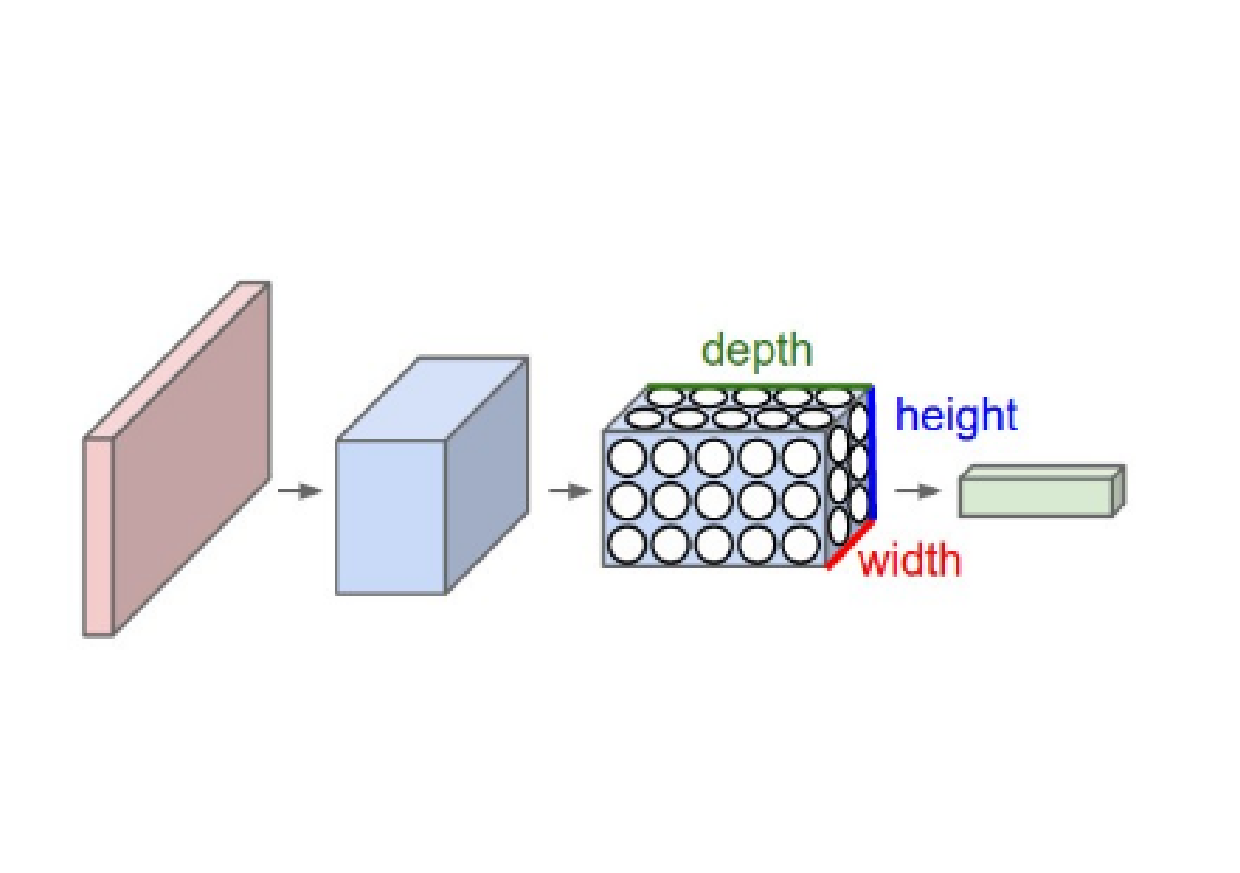
\includegraphics[height=6cm]{convolutional-neuron}
  \caption{A neuron in a convolutional network condensing image inputs into a 3D entity.~\cite{ref:}}
  \label{fig:cnn-neuron}
\end{figure}

Pooling is a transformation specific to convolutional neural networks: it combines clusters into a single entity to be used in the next layer, to condense and downsample previous operations with the intent to reduce parameters. This step assumes an image input and condenses the input into a 3-dimensional array, a convolutional neuron as seen in Figure~\ref{fig:cnn-neuron}. Max pooling, one of the most common types of pooling, is a downsampling function which takes the largest value from the prior cluster, effectively reducing the volume of data to process.  

The convolution process is usually paired with a concatenation step as well as an activation ReLU layer. ReLU stands for rectified linear unit, a process to introduce non-linearity in the CNN, effectively performing $f(x) = max(0, x)$.  

Finally, the fully connected (FC) layer flattens the transformed image matrix. During this FC layer, the softmax function normalizes the output to be between 0 and 1, as a sigmoid function, similar to a categorical probability distribution. In this case, it should be executed in the end to bring the model closer to indicating the probability and likelihood of hyperbolas. 

\subsection{Inception V3}

Inception V3 is a CNN of five convolutional layers, along with the typical max pooling and softmax functions. However, it differs from the standard design of CNN models by its successive stacking scattered throughout the model, between the convolutional layers, and is hence recognized as a deep training network.

Moreover, Inception extracts features at multiple levels, computing $1\times 1$, $3\times 3$, as well as $5 \times 5$ convolutional layers, which are concatenated afterwards to cover greater depths. This particularity of the model allows detection 

As such, the precision of this model can reach TODO.

The trade-off of such deep training is in its training speed: the processing of both the amount of stacking as well as the differing types of convolutional layers is expensive to compute. Although pre-trained Inception model is used, it contains TODO more layers per iteration of image training compared to Mobilenet, and TODO more than VGG.


As for the result of the model, the weights for Inception V3 are small, coming in at 96MB.



\subsection{MobileNet V2}


\subsection{VGG 19}
VGG 19 consists of five convolutional layers as well, $3 \times 3$ stacked on top of each other in increasing depth. Reducing volume size is handled by max pooling. Two fully-connected layers, each with 4,096 nodes are then followed by a softmax classifier (above).

"19" stand for the number of weight layers in the network.

The smaller networks converged and were then used as initializations for the larger, deeper networks — this process is called pre-training.

 % It only performs 3×33\times 33×3 convolutions and 2×22\times 22×2 pooling all the way through. It is currently the most preferred choice in the community for extracting features from images.

It is painfully slow to train.
    1. The network architecture weights themselves are quite large (in terms of disk/bandwidth).
Due to its depth and number of fully-connected nodes, VGG is over 533MB for VGG16 and 574MB for VGG19. This makes deploying VGG a tiresome task.
We still use VGG in many deep learning image classification problems; however, smaller network architectures are often more desirable (such as SqueezeNet, GoogLeNet, etc.).

Hence, the biggest drawbacks of VGG, despite its good depth and accuracy, would be hard to deploy onto Sensors and Software Inc’s GPR systems, and would only be something usable in EKKO Project, a post-processing software product.




% Here is a figure.  You MUST cite the figure in the text before it appears.
%
% I include an external picture here.  This picture is called don-hires.pdf.
% Notice how I do not specify the extension of the file.  pdfLaTeX knows
% about PDFs only, so get your pictures into that format.
%\begin{figure}
%  \centering
%  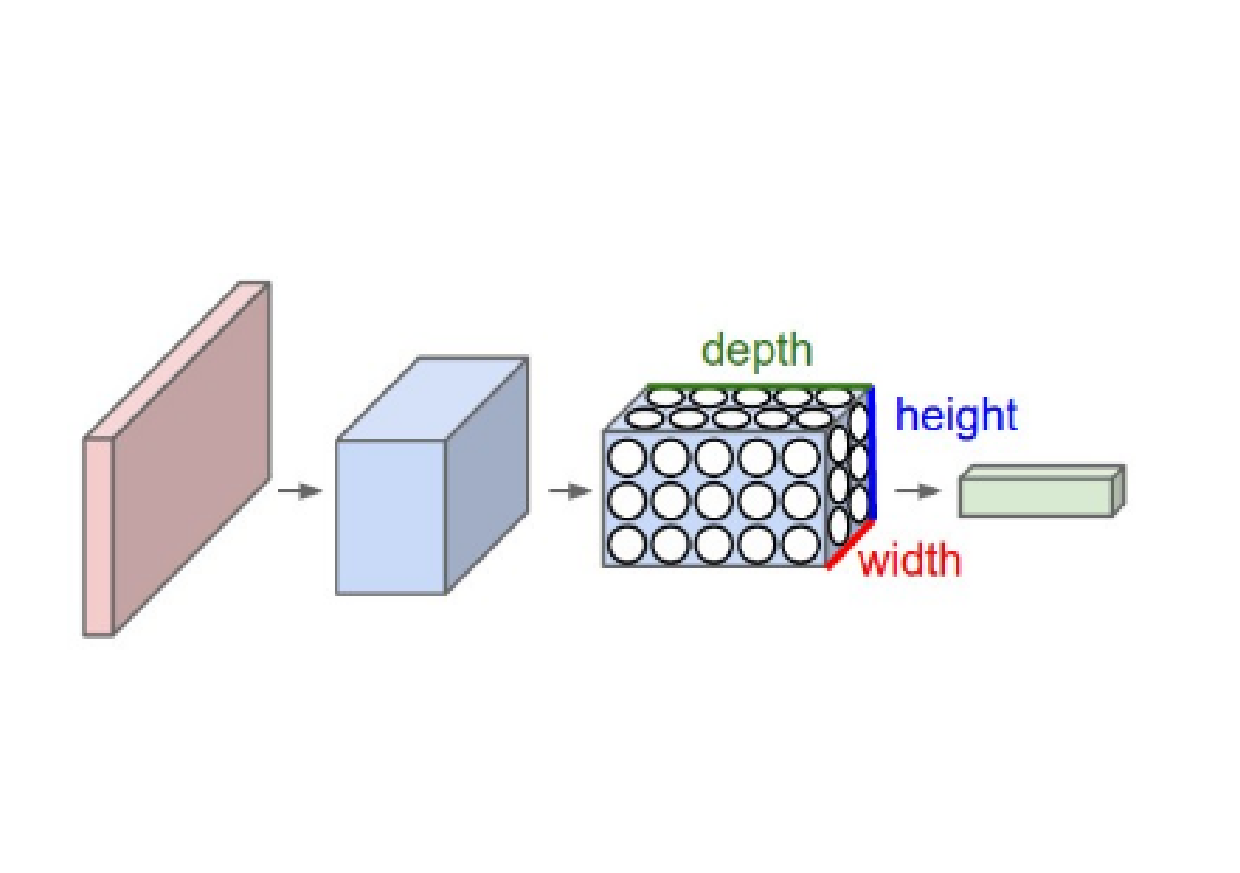
\includegraphics[height=3.0in]{convolutional-neuron}
%  \caption{A neuron in a convolutional network condensing image inputs into a 3D entity.~\cite{ref:}}
%\end{figure}

% Here is a table.  You MUST cite the table in the text before it appears
% in the document.
%\begin{table}
%  \caption{Typesetting special characters.}
%  \label{tbl:chars}
%  \centering
%  \begin{tabular}{|r|l|}
%    \hline
%    \multicolumn{1}{|c|}{\textbf{Name}} &
%    \multicolumn{1}{|c|}{\textbf{Symbol}} \\
%    \hline\hline
%    octothorpe   & \# \\
%    dollar sign  & \$ \\
%    percent sign & \% \\
%    ampersand    & \& \\
%    underscore   & \_ \\
%    left brace   & \{ \\
%    right brace  & \} \\
%    tilde        & \textasciitilde  \\
%    circumflex   & \textasciicircum \\
%    backslash    & \textbackslash   \\
%    \hline
%    inverted exclaimation & < \\
%    inverted question     & > \\
%    less than    & \textless \\
%    greater than & \textgreater \\
%    \hline
%  \end{tabular}
%\end{table}


% You must have a Conclusions section
\section{Conclusions}


% You must have a Recommendations section
\section{Recommendations}


%%%%%%%%%%%%%%%%%%%%%%%%%%%%%%%%%%%%%%%%%%%%%%%%%%%%%%%%%%%%%%%%%%%%%
%% BACK MATTER
%%%%%%%%%%%%%%%%%%%%%%%%%%%%%%%%%%%%%%%%%%%%%%%%%%%%%%%%%%%%%%%%%%%%%
%% \backmatter will make the \section commands ignore their numbering,
\backmatter

% Here, we insert a References section, which will be formatted properly.
% The list of works you have referenced should be specified in the preamble.
% In this template, the file is uw-wkrpt-bib.bib.
%
% Note, you will need to process the document in a certain order.  First,
% run LaTeX.  The % first pass will allow LaTeX to build a list of 
% references, it may % emit warning messages such as:
%   LaTeX Warning: Reference `app:gnugpl' on page 4 undefined on input line 277.
%   LaTeX Warning: There were undefined references.
% This is normal.  Now you run BiBTeX in order to generate the proper
% layout for the references.  After this, you run LaTeX once more.
\printbibliography[heading=bibintoc]


%%%%%%%%%%%%%%%%%%%%%%%%%%%%%%%%%%%%%%%%%%%%%%%%%%%%%%%%%%%%%%%%%%%%%
%% APPENDICES
%%%%%%%%%%%%%%%%%%%%%%%%%%%%%%%%%%%%%%%%%%%%%%%%%%%%%%%%%%%%%%%%%%%%%
%% \appendix will reset \section numbers and turn them into letters.
%%
%% Don't forget to refer to all your appendices in the main report.
\appendix


\end{document}
